\begin{figure}[ht]
 \centering
 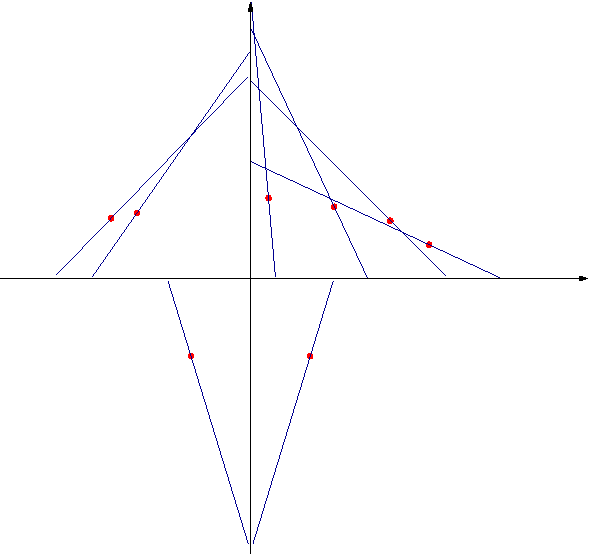
\includegraphics{Cconi1_1.pdf}
 % Cconi1_1.pdf: 302x283 pixel, 72dpi, 10.65x9.98 cm, bb=0 0 302 283
\caption{Construction de quelques points}
\label{fig:Cconi_1}
\end{figure} 
\begin{figure}[ht]
 \centering
\input{Cconi1_2.pdf_t}
\caption{Cercles de Chasles}
\label{fig:Cconi_2}
\end{figure}

\begin{enumerate}
 \item Voir la figure.
\item \begin{enumerate}
 \item Par définition, $0$, $P$, $I$, $Q$ est un rectangle donc les diagonales sont égales :
\begin{displaymath}
 OI = PQ =a+b
\end{displaymath}
 
\item Les coordonnées de $I$ s'obtiennent de la question précédente et de la définition de $\theta$, celles de $P$ et $Q$ s'en déduisent immédiatement :
\begin{align*}
 \text{coordonnées de $I$} &: ((a+b)\cos \theta , (a+b)\sin \theta) \\
 \text{coordonnées de $P$} &: ((a+b)\cos \theta , 0) \\
 \text{coordonnées de $Q$} &: (0 , (a+b)\sin \theta) 
\end{align*}
Par définition, $M$ est le barycentre de $(P,a)$ et de $(Q,b)$ donc
\begin{displaymath}
 (a+b)\overrightarrow{OM} = a\overrightarrow{OP} +  b\overrightarrow{OQ}
\end{displaymath}
Les coordonnées de $M$ sont donc
\begin{displaymath}
 (a\cos \theta , b \sin \theta)
\end{displaymath}
\item D'après la question précédente $\mathcal E$ est une ellipse.
\end{enumerate}
\item Voir la figure. Le point $I(\theta)$ est sur le cercle $\Gamma$, le point $J(\theta)$ est sur le cercle $\Gamma '$.
\begin{align*}
 \text{coordonnées de $I(\theta)$} &:  ((a+b)\cos \theta , (a+b)\sin \theta) \\
 \text{coordonnées de $J(\theta)$} &:  ((a-b)\cos \theta , (-a+b)\sin \theta) \\
 \text{coordonnées du milieu} &: (a\cos \theta , b\sin \theta) 
\end{align*}
On en déduit que le milieu est le point $M$ de la question 2.\newline
Les coordonnées de $\overrightarrow{I(\theta)J(\theta)}$ sont 
\begin{displaymath}
 (-2b\cos \theta , -2a \sin \theta)
\end{displaymath}
La tangente en $M(\theta)$ à l'ellipse $\mathcal E$ est portée par la dérivée dont les coordonnées sont :
\begin{displaymath}
 (-a\sin \theta , b\cos \theta)
\end{displaymath}
Ce vecteur est orthogonal à $\overrightarrow{I(\theta)J(\theta)}$ donc $(IJ)$ est la normale en $M$ à l'ellipse.
\end{enumerate}
